\documentclass[12pt,a4paper]{article}

% Essential Packages
\usepackage{amsmath}
\usepackage{geometry} % Adjust margins
\geometry{margin=1in}
\usepackage{graphicx} % For images
\usepackage{fancyhdr} % Custom headers and footers
\usepackage{titlesec} % Custom section titles
\usepackage{hyperref} % Hyperlinks
\usepackage{xcolor} % Colored text and links
\renewcommand{\thesubsection}{\alph{subsection}}

% Page Style


% Title Metadata
\title{Generative Transformers}
\author{Shaashvat Sekhar - WIDS 2k24}
\date{14 Feb 2025}

\begin{document}

\maketitle

\tableofcontents
\pagebreak
%%% Intro
\section{Introduction}

Transformers have emerged as one of the most versatile and powerful architectures in modern machine learning, driving advances in natural language processing and generative AI. Their ability to handle complex patterns and dependencies in data has made them foundational for large language models (LLMs) and other generative AI tools, which are rapidly shaping the future of technology and communication.\\

My motivation to do this project was to learn the underlying maths of a transformer, and to learn how to implement a basic generative transformer.\\

I thank my mentors Yash Sabale, and Aditya Neeraje for giving me this opportunity. \\

I thank the Analytics Club IIT Bombay, and WiDS 4.0 for connecting me with my mentors. \\

Shaashvat Sekhar


\pagebreak


%%% Updates from lab 4
\section{Week One}
In the first part of the project I familiarised myself with some python libraries and tools, and implemented gradient descent
\subsection{Familiarization, and insights}
\begin{itemize}
\item Python is a relatively easy language to write code in because it is a high-level language with english-like syntax and has lots of useful libraries for ML
\item NumPy has a feature called broadcasting which enables simultaneous element-wise operation on arrays of different shapes using vectorization. It enables fast matrix operations, making it useful for ML
\item Jupyter Notebooks are useful for creating projects because they have blocks which can be used to write and execute code systematically one step-at-a-time. They are also compatible with with LaTeX for equations, MatPlot Lib for visualising and all other python libraries
\end{itemize}

\subsection{Gradient Descent}
\begin{itemize}
\item Gradient Descent is a method to find a local minima of a continuous function. It is based on the principles of multivariable calculus, and concepts of partial derivatives and gradient.
\item The greatest descent of a function at a point $x$ is in the direction of: $-\nabla f$
\item By iteration of:
\subitem $x_{i+1} = x - \alpha * \nabla f(x_{i})$
\subitem Where $\alpha$ is called the "learning rate" and is a small positive constant, we can find a local minima of a functions (with some limitations)
\item $\alpha$ Can be dynamic to do gradient descent in less iterations (epochs). The "adam" optimizer uses this idea.
\item I used gradient descent to find a local minima of 
\subitem $f(x) = x^4 + x^2y^2 - y^2 + y^4 + 6$
\item This function has two local minimas, and gradient descent based on the initial position, ends up at (0, -7.07) or (0, 0.707)
\item This demonstrates that gradient descent can be used to find a local minima but not necesserily a global minima 
\item (code, outputs, visualisation: on next page)
\pagebreak
\begin{figure}[h!]
    \centering
    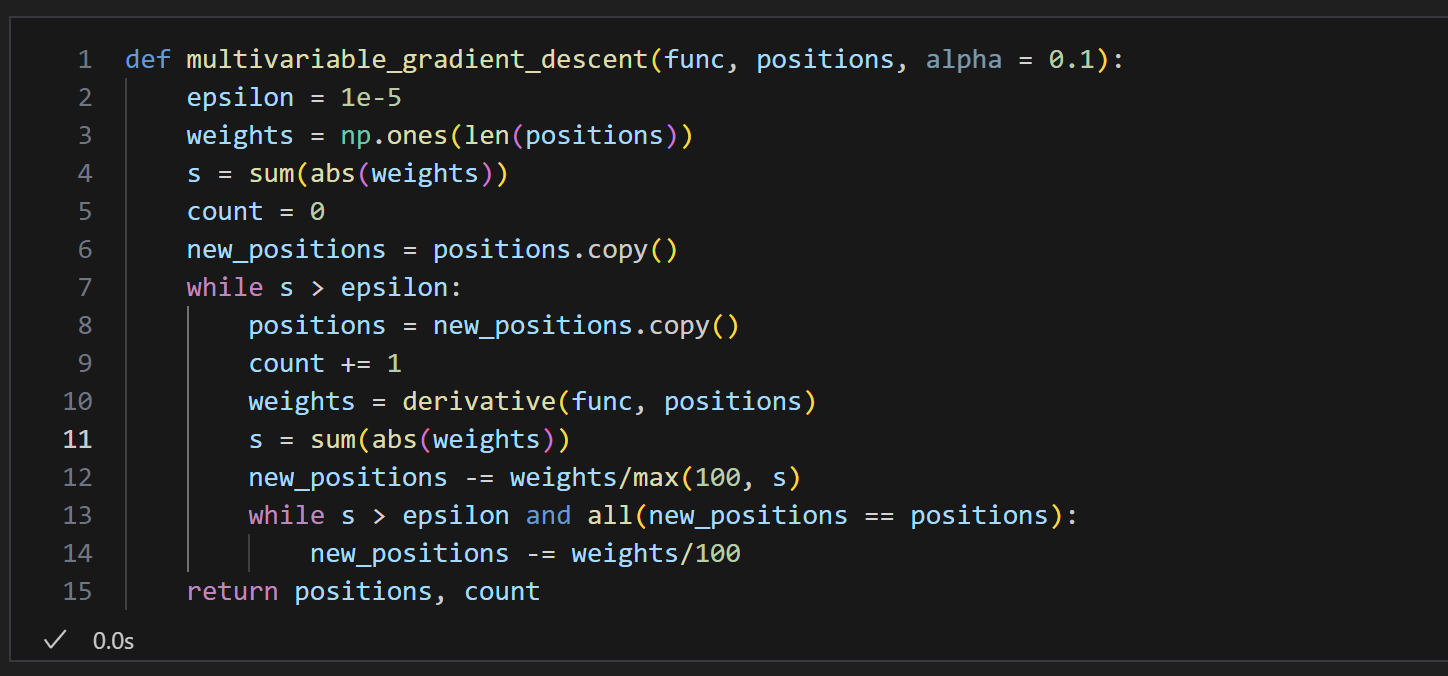
\includegraphics[width=0.8\textwidth]{grad1} 
    \caption{Gradient Descent Algo}
    \label{fig:example}
\end{figure}

\begin{figure}[h!]
    \centering
    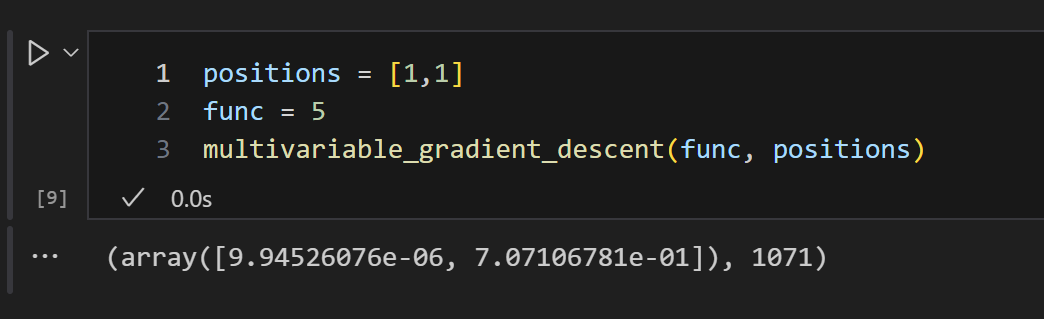
\includegraphics[width=0.8\textwidth]{grad2} 
    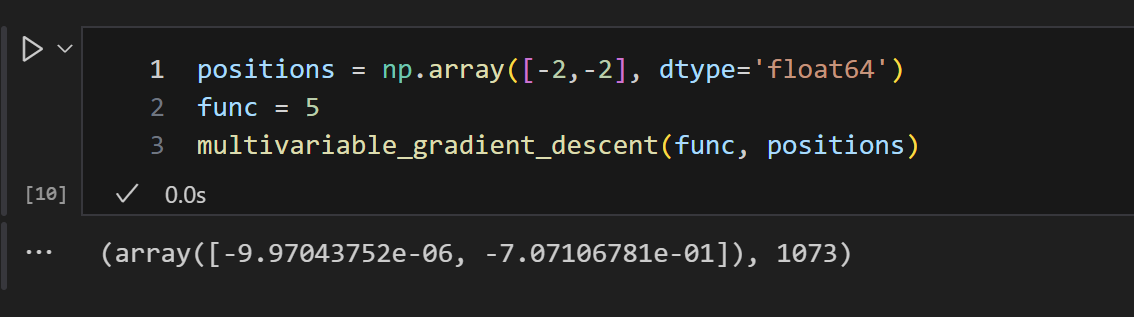
\includegraphics[width=0.8\textwidth]{grad3} 
    \caption{Gradient Descent Output}
    \label{fig:example}
\end{figure}
\begin{figure}[h!]
    \centering
    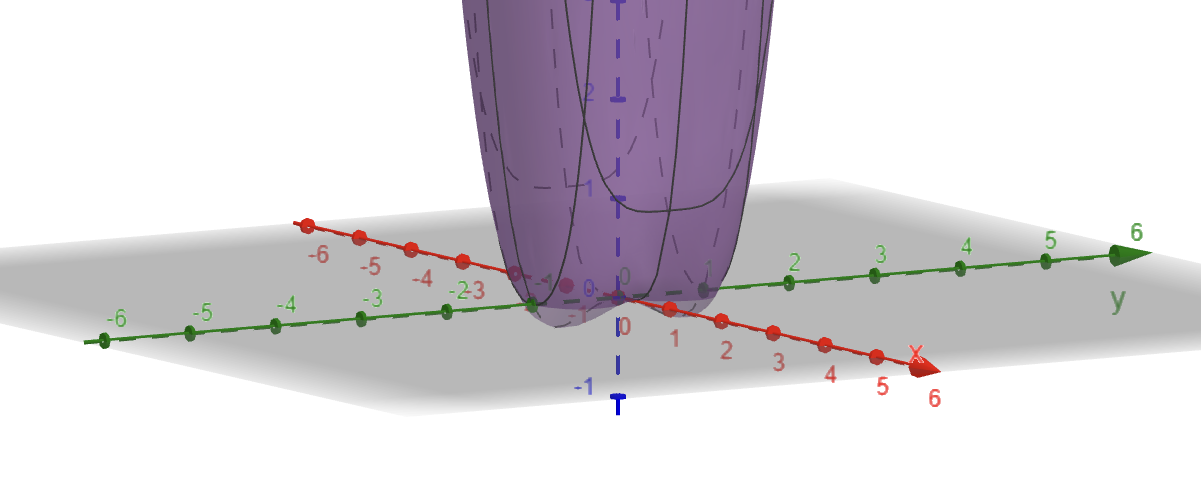
\includegraphics[width=0.8\textwidth]{grad4}
    \caption{Function Visualisation}
    \label{fig:example}
\end{figure}
\end{itemize}
\pagebreak
%%%%%%% WEEK 2
\section{Week Two}
In week two, I learned theory behind feedforward neural networks and used it to implement simple neural networks carrying out Boolean operations of two inputs
\subsection{Feedforward Neural Network}
\begin{itemize}
\item A feedforward neural network has multiple layers of "neurons" A-i
\item Each layer of neurons is created by a linear combination of the previous layer (inputs for layer-1) plus addition of bias, and finally a passthrough a non-linear activation function $ \sigma$
% Weighted Sum and Bias (Hidden Layer)
\[ z^{(1)} = W^{(1)}x + b^{(1)} \]
% Activation Function (Hidden Layer)
\[ a^{(1)} = \sigma(z^{(1)}) = \sigma(W^{(1)}x + b^{(1)}) \]
% Output Layer
\[ z^{(2)} = W^{(2)}a^{(1)} + b^{(2)} \]
% Output Layer Activation (e.g., Softmax)
\[ \hat{y} = \sigma_{\text{out}}(z^{(2)}) \]
\item Each neuron acts like a logistic regression. Having multiple neurons allows the model to "learn" different patterns. The "knowledge" is stored in the coefficients and biases which can create interesting effects because of the non-linear activation
\item The generalised expression:
% Matrix Form for Multiple Layers
\[ a^{(l)} = \sigma(W^{(l)}a^{(l-1)} + b^{(l)}), \quad \text{for } l = 2, 3, \dots, L \]
\[ a^{(0)} = x \quad \text{(input layer)}, \quad a^{(L)} = \hat{y} \quad \text{(output)} \]
\item 
% Loss Functions
% Mean Squared Error (MSE) for Regression
\[ \mathcal{L} = \frac{1}{N} \sum_{i=1}^{N} (\hat{y}_i - y_i)^2 \]

% Cross-Entropy Loss for Classification
\[ \mathcal{L} = -\sum_{i=1}^{N} y_i \log(\hat{y}_i) \]

% Backpropagation (Gradient Calculation)
\[ \frac{\partial \mathcal{L}}{\partial W^{(l)}} = \frac{\partial \mathcal{L}}{\partial a^{(l)}} \cdot \frac{\partial a^{(l)}}{\partial z^{(l)}} \cdot \frac{\partial z^{(l)}}{\partial W^{(l)}} \]

% Weight Update Rule (Gradient Descent)
\[ W^{(l)} := W^{(l)} - \eta \frac{\partial \mathcal{L}}{\partial W^{(l)}} \quad,\quad b^{(l)} := b^{(l)} - \eta \frac{\partial \mathcal{L}}{\partial b^{(l)}} \]

\end{itemize}

\subsection{Perceptrons}
\subsection{Perceptron implementation of AND}
\begin{itemize}
\item 
\end{itemize}


\end{document}

